\documentclass[12pt]{beamer}
\setbeamertemplate{navigation symbols}{}
\usetheme{Copenhagen}
\usepackage{listings}
\usepackage{xcolor}
\usepackage{graphicx}
\usepackage{hyperref}
\usepackage{multicol}
\graphicspath{ {imagenes/} }

\definecolor{codegreen}{rgb}{0,0.6,0}
\definecolor{codegray}{rgb}{0.5,0.5,0.5}
\definecolor{codepurple}{rgb}{0.58,0,0.82}
\definecolor{backcolour}{rgb}{0.95,0.95,0.92}

\lstdefinestyle{mystyle}{
    language=c++,
    backgroundcolor=\color{backcolour},   
    commentstyle=\color{codegreen},
    keywordstyle=\color{magenta},
    numberstyle=\tiny\color{codegray},
    stringstyle=\color{codepurple},
    basicstyle=\ttfamily\footnotesize,
    breakatwhitespace=false,         
    breaklines=true,                 
    captionpos=b,                    
    keepspaces=true,                 
    numbers=left,                    
    numbersep=5pt,                  
    showspaces=false,                
    showstringspaces=false,
    showtabs=false,                  
    tabsize=2
}

\lstset{style=mystyle}

\title{Strings}
\subtitle{Cadenas de caracteres en C++}
\author{Tomás Peiretti}
\date{}

\begin{document}

\maketitle

\begin{frame}{Strings}
    Los strings son objetos que representan una secuencia de caracteres, una \alert{cadena de caracteres}. Se los pueden pensar como un arreglo de caracteres, pero que incluyen una gran cantidad de métodos que facilitan las operaciones sobre ellos.
    
    \medskip

    Algunas operaciones:
    \begin{columns}
        \column{0.5\textwidth}\begin{itemize}
                \item \alert{clear()} permite vaciar el string
                \item \alert{size()} permite saber el tamaño del string
                \item \alert{copy()} permite copiar un string
                \item \alert{find()} permite encontrar la posicion de un elemento
            \end{itemize}
        \column{0.4\textwidth}
\includegraphics[width=\textwidth]{meme.jpeg}
    \end{columns}
\end{frame}

\begin{frame}[fragile]{String: métodos}
    Las operaciones que ofrecen los \alert{string} son métodos. Los métodos son similares a las funciones, pero se aplican sobre un string en particular:

\begin{lstlisting}[basicstyle=\tiny]
int main() {
    string cadena = "aedd practica strings";

    // imprimir el tamanio de cadena (21)
    cout << cadena.size() << endl;

    // imprimir la posicion donde comienza la cadena "practica" (5)
    cout << cadena.find("practica") << endl;

    // reemplazar "aedd" por "AEDD"
    cadena.replace(0,4,"AEDD");
    cout << cadena << endl; // imprime: AEDD practica strings

    // limpiar la cadena
    cadena.clear();
    cout << cadena << endl; // no imprime nada, porque la cadena quedo vacia
   
    return 0;
}
\end{lstlisting}
\end{frame}

\begin{frame}[fragile]{String: ejemplos}
\begin{lstlisting}[basicstyle=\tiny]
void recorrerCadena(string cadena) {
    // los strings pueden trabajarse como arreglos de caracteres, entonces:
    for (int i=0; i < cadena.size(); i++) {
        char caracter = cadena[i];
        cout<<"cadena[" << i << "] = " << caracter << endl;
    }
}
// por defecto, los strings pasan por copia!
// si deseamos modificarlo debemos indicar '&'
void invertirCadena(string & cadena) {
    int i=0, j=cadena.size()-1;
    while(i<j) {
        swap(cadena[i], cadena[j]);
        i++; j--;
    }
}

void ejemploOperadores() {
    string s1 = "gato", s2 = "perro", s3;
    // el operador '+' concatena dos strings
    cout << s1 + s2 + "321" << endl; // imprime: gatoperro321
    // es posible leer strings por teclado
    cin >> s3;
    // y tambien, los strings se pueden comparar con los operadores relacionales
    if (s3 == s2) {
        cout << "s3 es igual a s2" << endl;
    }
    if (s3 > s2) {
        cout << "s3 es lexicograficamente mayor que s2" << endl;
    }
}
\end{lstlisting}
\end{frame}


\begin{frame}[fragile]{String: ejemplo}
\begin{lstlisting}[basicstyle=\scriptsize]
// leer una linea entera y, 
// si en la linea se encuentra la frase "aedd es lo mejor" imprimir: "algo de ritmo y locura de datos"
int main() {

    string linea;
    // la funcion getline nos permite leer la linea entera
    getline(cin, linea);

    // el metodo find() nos permite saber si se encuentra la frase o no
    // si retorna npos, significa que no lo pudo encontrar
    if (linea.find("aedd es lo mejor") == string::npos) {
        cout << "la frase no se encuentra" << endl;
    }
    else {
        cout << "algo de ritmo y locura de datos" << endl;
    }

}
\end{lstlisting}
\end{frame}

\begin{frame}{Métodos de String}
    \centering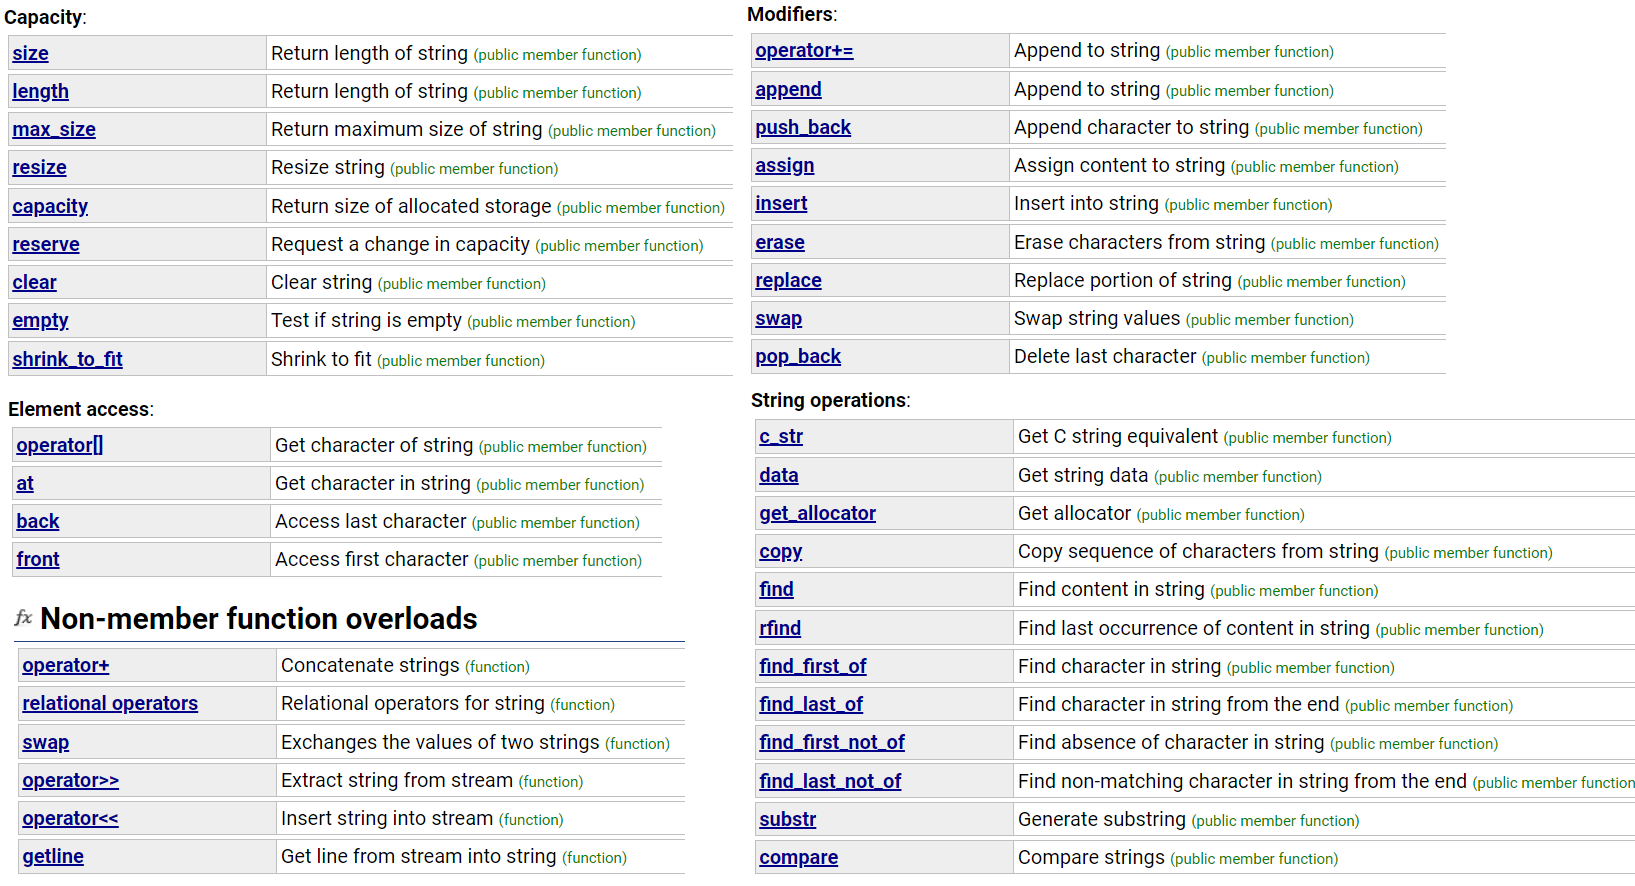
\includegraphics[width=\textwidth]{metodos.png}
    \centering\url{https://cplusplus.com/reference/string/string/}
\end{frame}

\begin{frame}{Ejercicios}
    \footnotesize\begin{multicols}{2}
        \begin{itemize}
            \item \href{https://omegaup.com/arena/problem/A-Contar-Letras/}{A Contar Letras}
            \item \href{https://omegaup.com/arena/problem/Ola-ivan/}{Ola ivan}
            \item \href{https://omegaup.com/arena/problem/Bajando-los-caracteres/}{Bajando los caracteres}
            \item \href{https://omegaup.com/arena/problem/Invertir-Palabra/}{Invertir Palabra}
            \item \href{https://omegaup.com/arena/problem/BIT_DE_PARIDAD/}{Bit de paridad}
            \item \href{https://omegaup.com/arena/problem/Buscando-la-inicial/}{Buscando la inicial}
            \item \href{https://omegaup.com/arena/problem/SEGUETAV/}{SEGUETAV}
            \item \href{https://omegaup.com/arena/problem/Frecuencia-de-una-letra/}{Frecuencia de una letra}
            \item \href{https://omegaup.com/arena/problem/Creo-que-ya-funciona/}{Creo que ya funciona}
            \item \href{https://omegaup.com/arena/problem/Recortando-palabras/}{Recortando palabras}
            \item \href{https://omegaup.com/arena/problem/Dias-de-la-actualidad/}{Dias de la actualidad}
            \item \href{https://omegaup.com/arena/problem/Cuenta-Cadenas/}{Cuenta cadenas}
            \item \href{https://omegaup.com/arena/problem/Abreviando-palabras/}{Abreviando palabras}
            \item \href{https://omegaup.com/arena/problem/Encontrando-Anagramas/}{Encontrando Anagramas}
            \item \href{https://omegaup.com/arena/problem/El-caballo-de-John-Carter/}{El caballo de John Carter}
            \item \href{https://omegaup.com/arena/problem/Bailando-con-Cesar/}{Bailando con Cesar}
        \end{itemize}
    \end{multicols}
\end{frame}

\end{document}